%
% This is the LaTeX template file for lecture notes for EE 382C/EE 361C.
%
% To familiarize yourself with this template, the body contains
% some examples of its use.  Look them over.  Then you can
% run LaTeX on this file.  After you have LaTeXed this file then
% you can look over the result either by printing it out with
% dvips or using xdvi.
%
% This template is based on the template for Prof. Sinclair's CS 270.

\documentclass[twoside]{article}
\usepackage{graphics}
\usepackage{graphicx}
\usepackage{algorithm}
\usepackage{mathtools}
\usepackage{mathptmx}
\usepackage{algpseudocode}
\setlength{\oddsidemargin}{0.25 in}
\setlength{\evensidemargin}{-0.25 in}
\setlength{\topmargin}{-0.6 in}
\setlength{\textwidth}{6.5 in}
\setlength{\textheight}{8.5 in}
\setlength{\headsep}{0.75 in}
\setlength{\parindent}{0 in}
\setlength{\parskip}{0.1 in}

%
% The following commands set up the lecnum (lecture number)
% counter and make various numbering schemes work relative
% to the lecture number.
%
\newcounter{lecnum}
\renewcommand{\thepage}{\thelecnum-\arabic{page}}
\renewcommand{\thesection}{\thelecnum.\arabic{section}}
\renewcommand{\theequation}{\thelecnum.\arabic{equation}}
\renewcommand{\thefigure}{\thelecnum.\arabic{figure}}
\renewcommand{\thetable}{\thelecnum.\arabic{table}}

%
% The following macro is used to generate the header.
%
\newcommand{\lecture}[4]{
   \pagestyle{myheadings}
   \thispagestyle{plain}
   \newpage
   \setcounter{lecnum}{#1}
   \setcounter{page}{1}
   \noindent
   \begin{center}
   \framebox{
      \vbox{\vspace{2mm}
    \hbox to 6.28in { {\bf EE 382C/361C: Multicore Computing
                        \hfill Fall 2016} }
       \vspace{4mm}
       \hbox to 6.28in { {\Large \hfill Lecture #1: #2  \hfill} }
       \vspace{2mm}
       \hbox to 6.28in { {\it Lecturer: #3 \hfill Scribe: #4} }
      \vspace{2mm}}
   }
   \end{center}
   \markboth{Lecture #1: #2}{Lecture #1: #2}
   %{\bf Disclaimer}: {\it These notes have not been subjected to the
   %usual scrutiny reserved for formal publications.  They may be distributed
   %outside this class only with the permission of the Instructor.}
   \vspace*{4mm}
}

%
% Convention for citations is authors' initials followed by the year.
% For example, to cite a paper by Leighton and Maggs you would type
% \cite{LM89}, and to cite a paper by Strassen you would type \cite{S69}.
% (To avoid bibliography problems, for now we redefine the \cite command.)
% Also commands that create a suitable format for the reference list.
\renewcommand{\cite}[1]{[#1]}
\def\beginrefs{\begin{list}%
        {[\arabic{equation}]}{\usecounter{equation}
         \setlength{\leftmargin}{2.0truecm}\setlength{\labelsep}{0.4truecm}%
         \setlength{\labelwidth}{1.6truecm}}}
\def\endrefs{\end{list}}
\def\bibentry#1{\item[\hbox{[#1]}]}

%Use this command for a figure; it puts a figure in wherever you want it.
%usage: \fig{NUMBER}{SPACE-IN-INCHES}{CAPTION}
\newcommand{\fig}[3]{
			\vspace{#2}
			\begin{center}
			Figure \thelecnum.#1:~#3
			\end{center}
	}
% Use these for theorems, lemmas, proofs, etc.
\newtheorem{theorem}{Theorem}[lecnum]
\newtheorem{lemma}[theorem]{Lemma}
\newtheorem{proposition}[theorem]{Proposition}
\newtheorem{claim}[theorem]{Claim}
\newtheorem{corollary}[theorem]{Corollary}
\newtheorem{definition}[theorem]{Definition}
\newenvironment{proof}{{\bf Proof:}}{\hfill\rule{2mm}{2mm}}

% **** IF YOU WANT TO DEFINE ADDITIONAL MACROS FOR YOURSELF, PUT THEM HERE:

\begin{document}
%FILL IN THE RIGHT INFO.
%\lecture{**LECTURE-NUMBER**}{**DATE**}{**LECTURER**}{**SCRIBE**}
\lecture{1}{September 22}{Vijay Garg}{Chuiye Kong}
%\footnotetext{These notes are partially based on those of Nigel Mansell.}

% **** YOUR NOTES GO HERE:

% Some general latex examples and examples making use of the
% macros follow.  
%**** IN GENERAL, BE BRIEF. LONG SCRIBE NOTES, NO MATTER HOW WELL WRITTEN,
%**** ARE NEVER READ BY ANYBODY.
\section{Introduction}
%Students in EE 382C are required to scribe lecture notes for one lecture.
%These lecture notes will be done using the document processing system called Latex.
%We have posted the file {\em scribe.tex} on the Canvas system. You can run {\tt pdflatex}
%on that file to generate {\em scribe.pdf}. The remaining document shows usage of
%some of the commands in Latex.
\indent In this lecture, we first go over the puzzle of merging algorithm, then we discuss Monitor.
\indent Outline is shown as follows:
\begin{enumerate}
	\item Sequential and two parallel solutions for Merging algorithm (puzzle)
	\item Synchronization
	\item Monitor
	\item Problems using monitor
\end{enumerate}


\section{Merging Puzzle}
As shown in Figure \ref{fig:sortedarrays}, the problem is to merge two sorted array into one sorted array. 

\begin{figure}[ht]
  \centering
  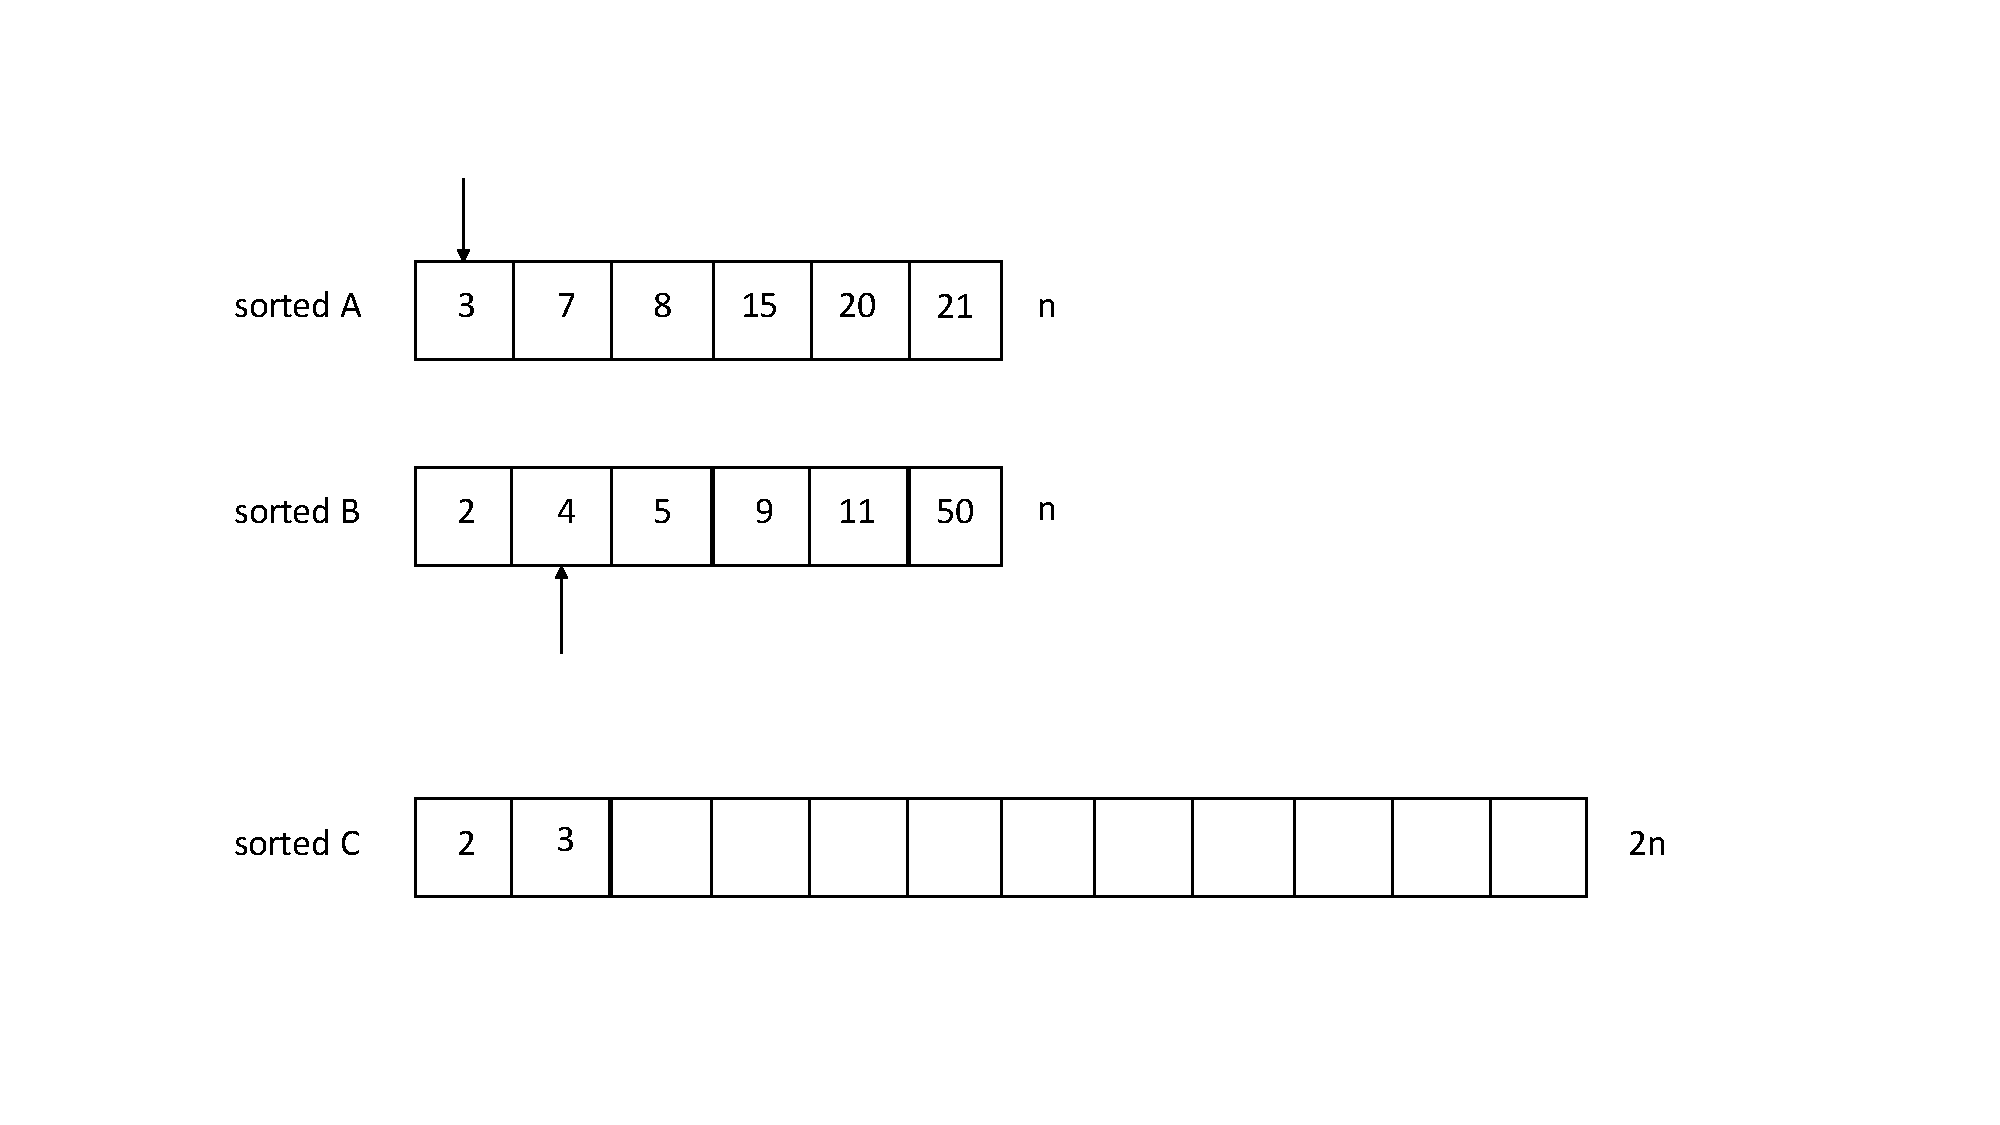
\includegraphics[height=0.250\textheight,width=0.750\linewidth]{./sortedarray.pdf} 
  \caption{Merging Sorted Arrays}
  \label{fig:sortedarrays}
\end{figure}

The sequential solution is using two pointers to point each array and compare the two pointed array items. The smaller item will be put into array C and its point will move to next element in the array. The timing complexity T(n) of this solution is O(n) and the work W(n) is O(n) as well. 

\subsection{Parallel Solution I}
Select a key element in A (for example, we can choose 15), then array A will be split into left and right, which are annotated as A.left and A.right in Figure \ref{fig:p1}. Do the binary search for 15 (the key element we selected) in array B. B will be divided up into the  \textless 15 part and \textgreater 15 part, and allocated on the left side of the key element and on right side of it. The time complexity T(n) is O(log(n)log(n)) and work is O(nlog(n)log(n)). 

\begin{figure}[ht]
  \centering
  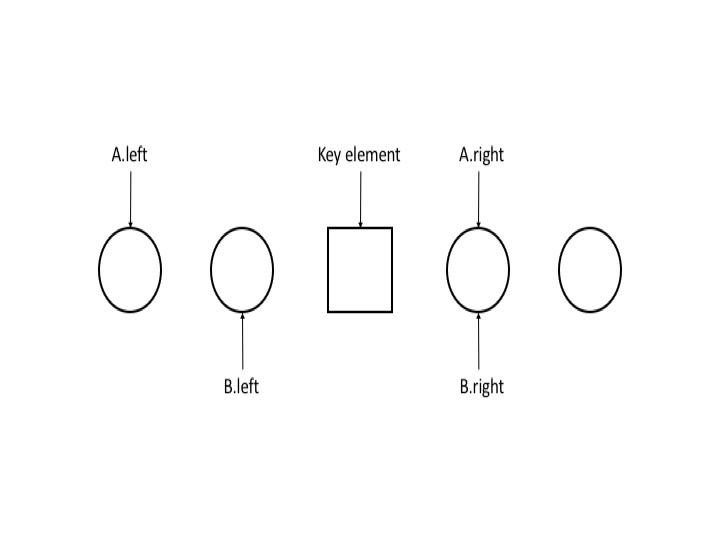
\includegraphics[height=0.250\textheight,width=0.750\linewidth]{./p1.jpg} 
  \caption{Binary Search for Key Element}
  \label{fig:p1}
\end{figure}

\subsection{Parallel Solution II}
Now, we define rank(x), which is equal to the sum of the number of elements in A less than X and the number of elements in B less than X. For example, if we are looking for rank(A[j]), then the answer is j + binary search to find rank of A[j] in B, where j is the index in A as shown in Figure \ref{fig:p2}. The timing complexity of this algorithm is O(log) and the work is O(nlog(n)).

\begin{figure}[ht]
  \centering
  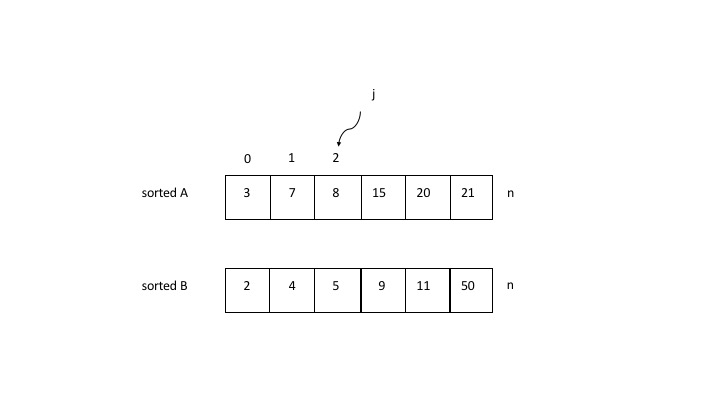
\includegraphics[height=0.250\textheight,width=1.0\linewidth]{./p2.jpg} 
  \caption{Rank example of A[j]}
  \label{fig:p2}
\end{figure}

\section{Synchronization}
As far as we know, Synchronization can be used for mutual exclusion and conditional synchronization. To achieve mutual exclusion, waiting thread deploys two methods, which are busy-wait and sleep. Conditional synchronization is needed when a thread must wait for a certain condition to become true. Example is shown in Figure \ref{fig:syn}. We can see foo() has to do v() before T2 go to bar(). The drawbacks of using semaphore to achieve synchronization can be summarized into two points. First, it is hard to tell the difference between mutual exclusion and conditional synchronization. Secondly, the order of acquire() matters, as it may cause deadlock (refer back to Semaphore lecture). It is not very reasonable to let programmers take care of this ordering problem. Therefore, we will introduce Monitor in the next section. 

\begin{figure}[ht]
  \centering
  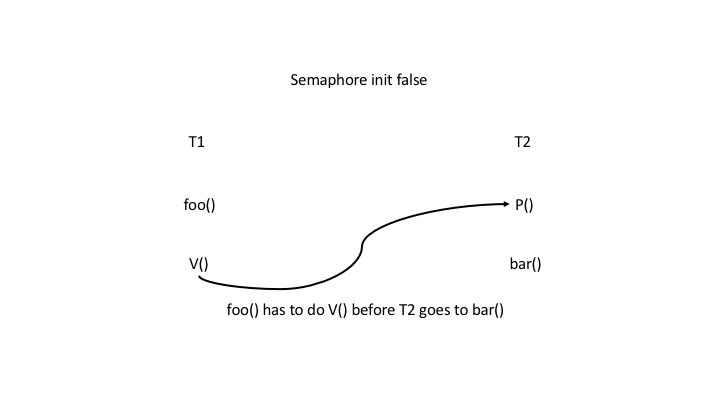
\includegraphics[height=0.250\textheight,width=1.0\linewidth]{./syn.jpg} 
  \caption{Conditional Synchronization Example}
  \label{fig:syn}
\end{figure}


\section{Monitor}
We can use Monitor to replace Semaphore for both mutual exclusion and conditional synchronization purposes. There are two types of Monitors we can use, which are synchronized and reenetrant lock. A conditional variable has two operations: \textit{wait} and \textit{notify} (also called \textit{signal}). In Java, the threads usually wait for the condition as shown in Algorithm \ref{alg:while}.
\begin{algorithm}
\caption{Conditional Wait.}
\begin{algorithmic}[1]
\State while (!B) \{
\State \indent wait();
\State \} 
\end{algorithmic}
\label{alg:while}
\end{algorithm}
\newline
\textit{notify} is used to wake up one thread and \textit{notifyAll} is used to wake up all threads in the waiting queue. \textit{Wait} inserts the thread in the wait queue. 
\newline
\textit{Monitor Invariant} is defined as: at most one thread can be in the monitor at any given time. A example of monitor is shown in Figure \ref{fig:monitor}.

\begin{figure}[ht]
  \centering
  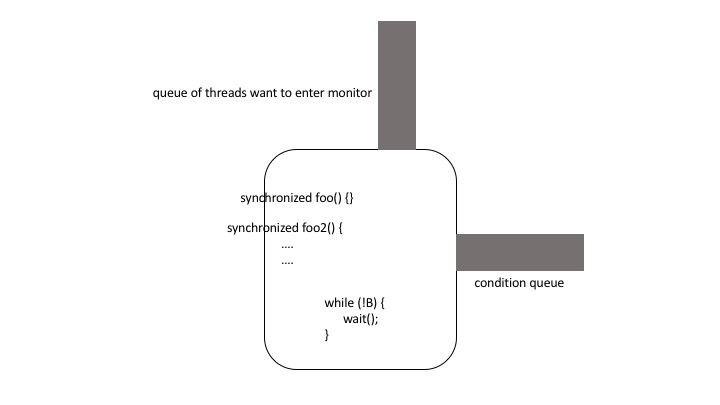
\includegraphics[height=0.250\textheight,width=1.0\linewidth]{./monitor.jpg} 
  \caption{Monitor Example}
  \label{fig:monitor}
\end{figure}

Wait queue and condition queue may both have ready thread that can enter the monitor. The problem here is: which thread should continue after the notify operation. There are two possible answers:

\begin{enumerate}
	\item One of threads that was waiting on the condition variable continues execution. Monitors that follow this rule are called \textit{Hoare} monitors (or, \textit{signal-and-wait monitors}).
	\item The thread that made the notify call continues its execution. When this thread goes out of the monitor, then other threads can enter the monitor. This is the semantics followed in Java and is called \textit{signal-and-continue}.
\end{enumerate}

\section{Problems Using Monitor}
\subsection{Producer and Consumer}
The buffer is shown in Figure \ref{fig:pc}. The BoundedBufferMonitor is used for one producer and one consumer, which has two entry methods: \textit{deposit} and \textit{fetch}. If a thread is executing the method \textit{deposit} or \textit{fetch}, then no other thread can execute \textit{deposit} or \textit{fetch}. The code of BoundedBufferMonitor is shown in \cite{1}. This code works correctly only when there is exactly one producer and one consumer. The modified MBoundedBufferMonitor is designed to solve this issue and it can be found at \cite{2}.
\begin{figure}[ht]
  \centering
  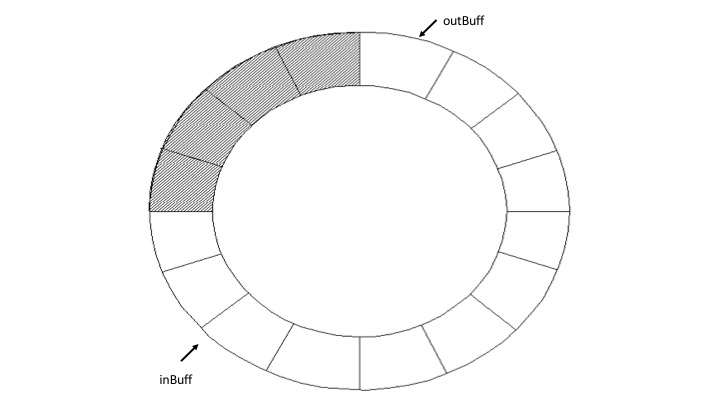
\includegraphics[height=0.250\textheight,width=1.0\linewidth]{./pc.jpg} 
  \caption{Producer and Consumer}
  \label{fig:pc}
\end{figure}
\subsection{Dining Philosophers}
The code for using Monitor to solve Dining Philosophers is demoed in \cite{3}. The code guarantees the mutual exclusion and deadlock-free, however, it does not guarantee freedom from starvation.  
\subsection{Nested Monitor}
Nested monitor can cause deadlock problem when a thread waits for a condition inside a nested monitor. For example, a thread t1 is inside a monitor for an object \textit{object1} and calls a synchronized method for another object \textit{object2}. If the thread invokes a \textit{wait()} inside it, then it will release the lock on \textit{object2}. However, it will continue to hold the monitor lock of \textit{object1}. If we have a thread t2 can notify thread t1, but thread t2 needs the lock of \textit{object1}, a deadlock appears. 

\section*{References}
\beginrefs
\bibentry{1} https://github.com/vijaygarg1/UT-Garg-EE382C-EE361C-Multicore/blob/master/chapter3-
\\synchronization\_primitives/BoundedBufferMonitor.java
\bibentry{2} https://github.com/vijaygarg1/UT-Garg-EE382C-EE361C-Multicore/blob/master/chapter3-
\\synchronization\_primitives/MBoundedBufferMonitor.java
\bibentry{3} https://github.com/vijaygarg1/UT-Garg-EE382C-EE361C-Multicore/blob/master/chapter3-
\\synchronization\_primitives/DiningMonitor.java
\endrefs


\end{document}





